\newpage
\section{Entwurf eines Task Scheduling Verfahrens}\label{sec:Gesamtkonzept}
Um die in Abschnitt \ref{sec:Datenerfassung} und \ref{sec:Datenverarbeitung} beschriebenen Teilsysteme zu einem lauffähigen Programm zusammenzuführen, wird ein Konzept benötigt, das es erlaubt, einzelne Aufgaben in regelmäßigen Intervallen auszuführen. Dieses Konzept kann durch die Verwendung eines TaskSchedulers realisiert werden, der die zeitliche Planung und Ausführung der einzelnen Aufgaben gemäß den festgelegten Intervallen steuern und verwalten kann. Hierzu werden unter dem \textit{HM.TimerBasedScheduler} Verzeichnis folgende Klassen angelegt. (Siehe Abbildung \ref{fig:TimerBasedScheduler}) 
\begin{center}
    \begin{figure}[h!]
        \centering
        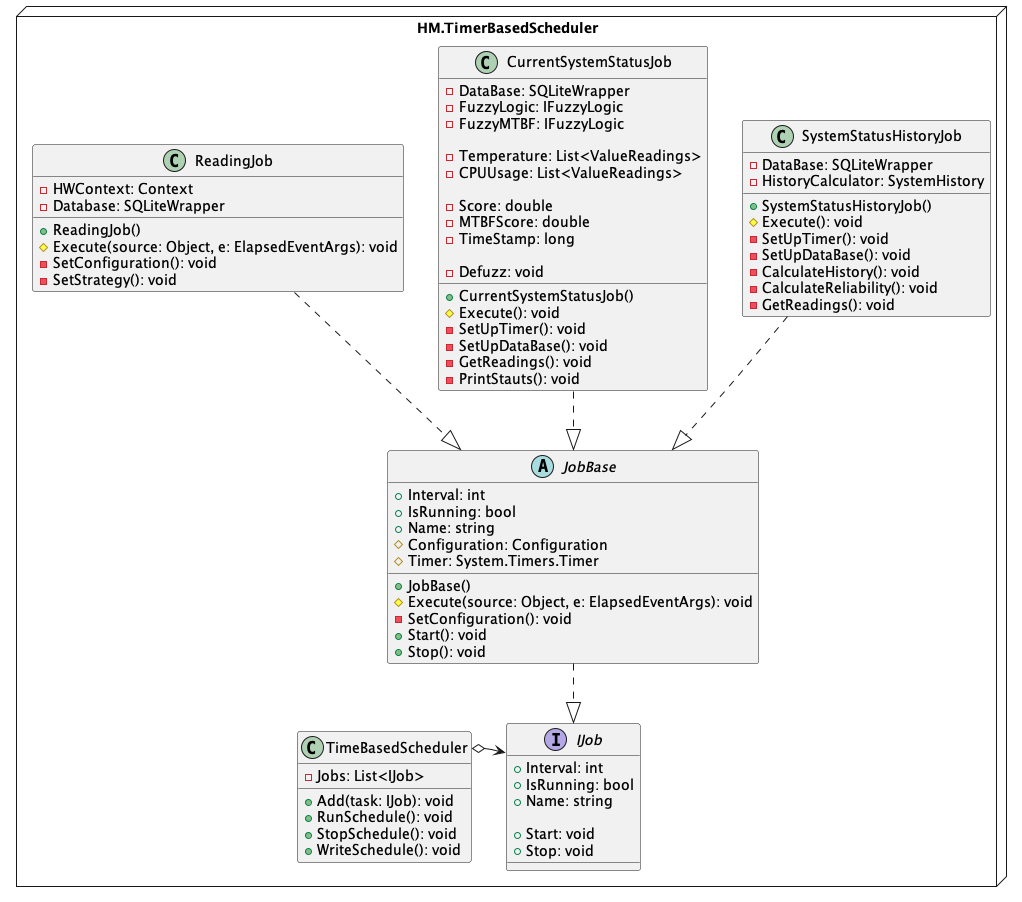
\includegraphics[width=1\textwidth]{HMTimerBasedScheduler.png}
        \caption{Architektur des Taskscheduler}
        \label{fig:TimerBasedScheduler}
    \end{figure}
\end{center}
Die Basis des Schedulers ist die \textit{TimerBasedScheduler} Klasse. In dieser können verschiedene Aufgaben zum Zeitplan hinzugefügt werden. Zudem kann der Scheduler in dieser Klasse gestartet und gestopt werden. Um zur Laufzeit des Programms eine Übersicht über die laufenden Aufgaben zu haben wird der \textit{TimerBasedScheduler} Klasse eine Funktion zur visualisierung des Zeitplans in der Console hinzugefügt.\\
Die Schnittstelle zu einer bestimmten Aufgabe, im weiteren als Job bezeichnet, wird über das \textit{IJob} Interface definiert. Dieses definiert die von der \textit{TimerBasedScheduler} Klasse verwendeten Funktionen und Variablen. Aus diesem wird anschließend die abstrakte \textit{JobBase} Klasse abgeleitet, aus welcher anschließend die Eigentlichen Jobs Abgeleitet werden können. Die \textit{JobBase} Klasse liefert alle Basisfunktionen und Variablen, welche in jedem Job verwendet werden. Die verwendung einer Basisklasse verhindert Codedublikation und erleichtert durch eine vordefinierte Struktur das Programmieren der Spezifischen Jobs. \\

\subsubsection*{ReadingJob}

\subsubsection*{CurrentStatusJob}

\subsubsection*{SystemStatusHistoryJob}